\hsection{Entity Relationship Diagrams}%
\label{sec:entitisAttrsErd}%
We now know that entity types with their attributes basically correspond to datastructures in programming.
They form one element of the conceptual model.
But how do we actually write them down?
How do we specify them?

For this, a graphical notation has been introduced:
\glsreset{ERD}\Pglspl{ERD} are the most commonly used tool to model the entity types and their relationships in a \db~\cite{C2002ERMHEFTALL,C1975TRMTAUVOD,C1976TERMTAUVOD,KW2012ASHOTEDAIM,WF1995DHQDM,B1990CMERMO}.
There exists a wide variety of graphical notations that can be used for \pglspl{ERD}.
The original notations by \citeauthor{B1969DSD}~\cite{B1969DSD} and \citeauthor{C1975TRMTAUVOD}~\cite{C1975TRMTAUVOD,C1976TERMTAUVOD} are still in use, the more comprehensive and standardized \pgls{IDEF1X} syntax~\cite{FIPSPUB184,ISOIECIEEE2012ITMLP2SASFII}, and the \glsreset{UML}\pgls{UML}~\cite{OMG2017OUMLOU,RMHOSMUUIIIIOPPTRS1997UNG,BRJ1999TUMLRM}.
Indeed, there are many different flavors of diagrams that can serve as \pglspl{ERD}.
\Citeauthor{S2024D:CDMERDE}~\cite{S2024D:CDMERDE}, for example, presents nine slightly different variations.
\Citeauthor{SS2005EIDDDFDB:CDDRAAML}~\cite{SS2005EIDDDFDB:CDDRAAML} has two baseline variants, including several slight variations of a \pgls{UML}-based approach~(which is not listed in~\cite{S2024D:CDMERDE}).
The notation used by \citeauthor{V1999C5DMS:CDUTERM}~\cite{V1999C5DMS:CDUTERM} is yet again slightly different.
Therefore, \pglspl{ERD} may look slightly different depending on who drew them and which tools they used.
However, understanding them is not really hard, so these differences are not that important.

\begin{figure}%
\centering%
%
\subfloat[][%
We open the \yEd\ editor and click on the \menu{Entity Relationship} tab in the \menu{Palette} view on the right-hand side.%
\label{fig:yedErdEntitiesA01scrollToErd}%
]{\tightbox{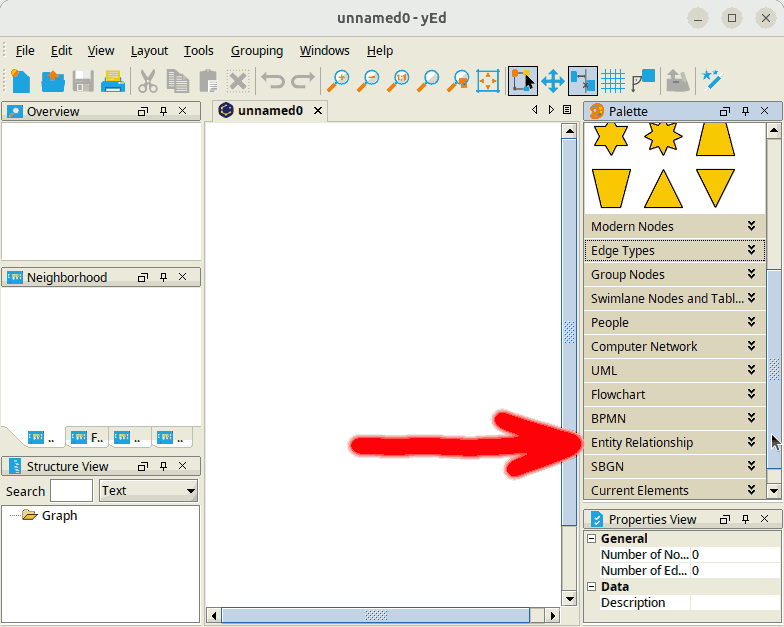
\includegraphics[width=0.48\linewidth]{\currentDir/yedErdEntitiesA01scrollToErd}}}%
%
\floatSep%
%
\subfloat[][%
We can now click on the \menu{Entity} symbol and drag it into the empty document.%
\label{fig:yedErdEntitiesA02entity}%
]{\tightbox{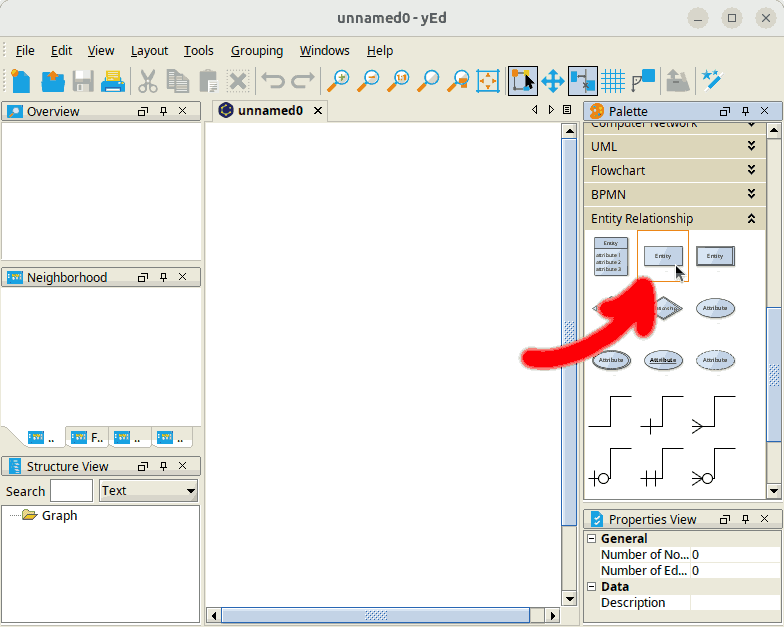
\includegraphics[width=0.48\linewidth]{\currentDir/yedErdEntitiesA02entity}}}%
%
\floatRowSep
%
\subfloat[][%
We dragged the entity symbol into the diagram document.%
\label{fig:yedErdEntitiesA03dragEntity}%
]{\tightbox{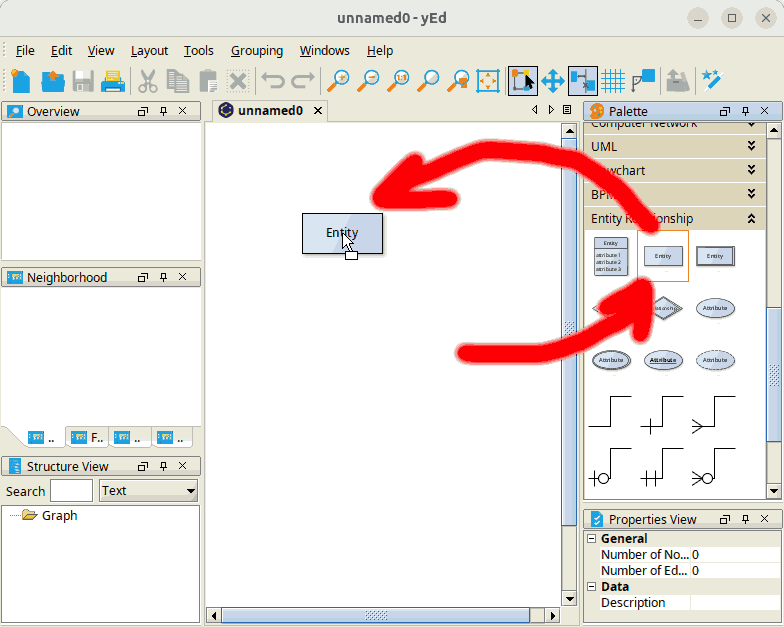
\includegraphics[width=0.48\linewidth]{\currentDir/yedErdEntitiesA03dragEntity}}}%
%
\floatSep
%
\subfloat[][%
We double-click into the new entity symbol in order to edit its name.%
\label{fig:yedErdEntitiesA04doubleClickName}%
]{\tightbox{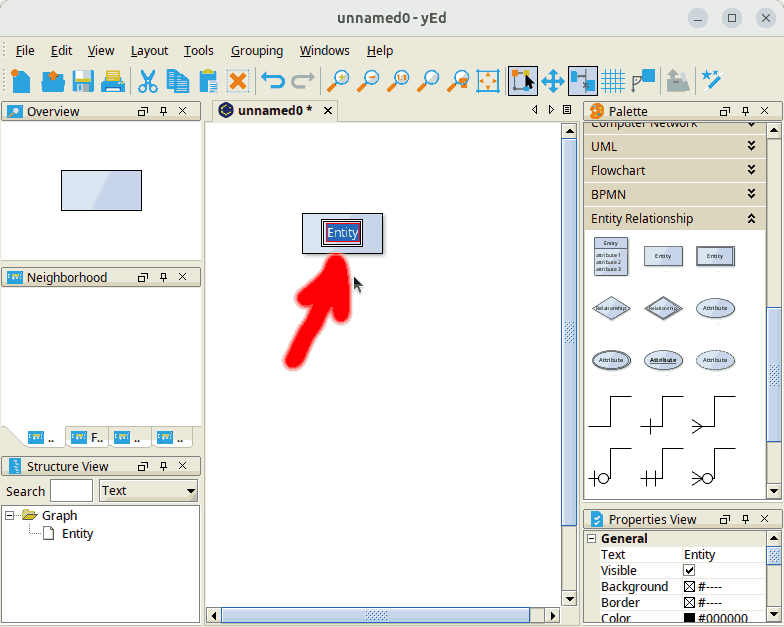
\includegraphics[width=0.48\linewidth]{\currentDir/yedErdEntitiesA04doubleClickName}}}%
%
\floatRowSep
%
\subfloat[][%
We change the entity name to \inQuotes{Student} and press \keys{\enter}.%
\label{fig:yedErdEntitiesA05changeNameToStudent}%
]{\tightbox{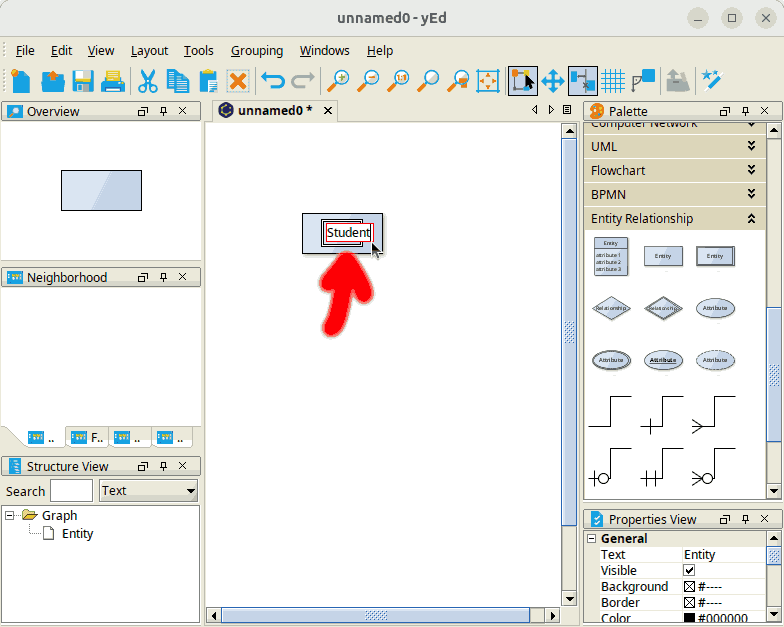
\includegraphics[width=0.48\linewidth]{\currentDir/yedErdEntitiesA05changeNameToStudent}}}%
%
\floatSep
%
\subfloat[][%
The name has changed. We now click on the \menu{Attribute} symbol in the element palette.%
\label{fig:yedErdEntitiesA06nameIsStudentSelectAttribute}%
]{\tightbox{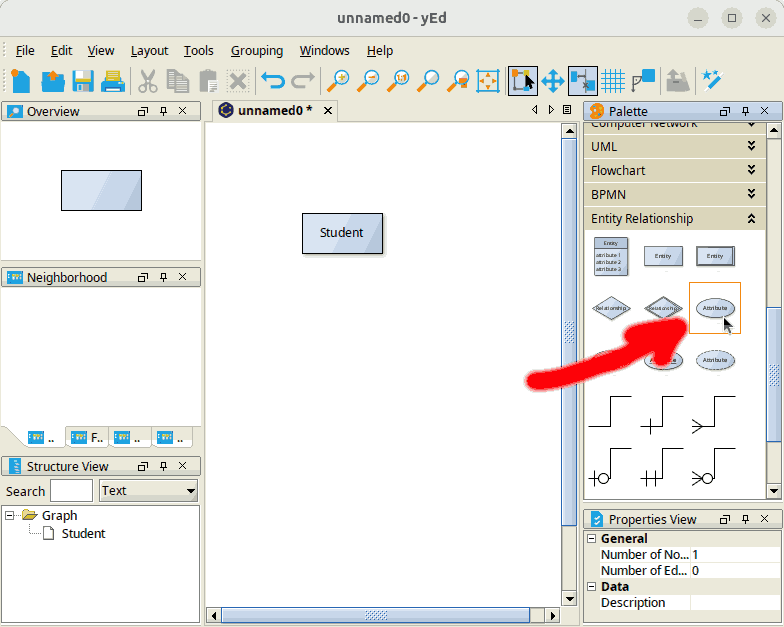
\includegraphics[width=0.48\linewidth]{\currentDir/yedErdEntitiesA06nameIsStudentSelectAttribute}}}%
%
\caption{Drawing an \pgls{ERD} for the \emph{Student} entity using \yEd.}%
\label{fig:yedErdEntitiesA:A}%
\end{figure}%
%
\begin{figure}%
\ContinuedFloat%
\centering%
%
\subfloat[][%
We drag the attribute symbol into our document.%
\label{fig:yedErdEntitiesA07dragAttribute}%
]{\tightbox{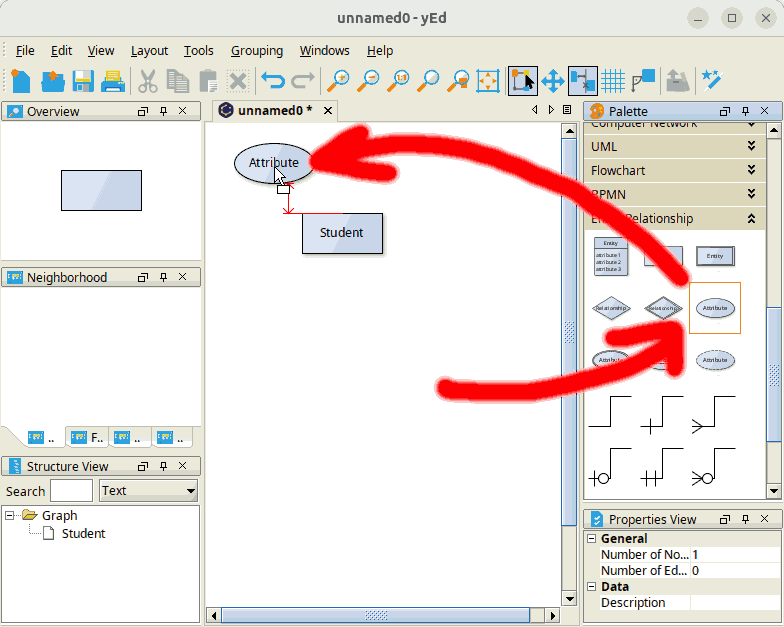
\includegraphics[width=0.48\linewidth]{\currentDir/yedErdEntitiesA07dragAttribute}}}%
%
\floatSep%
%
\subfloat[][%
We double-click into it to change its name.%
\label{fig:yedErdEntitiesA08doubleClickName}%
]{\tightbox{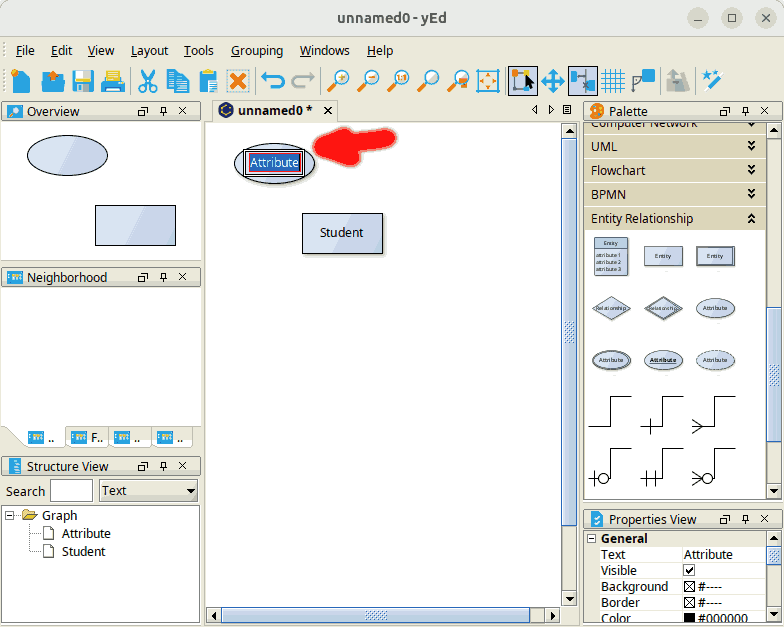
\includegraphics[width=0.48\linewidth]{\currentDir/yedErdEntitiesA08doubleClickName}}}%
%
\floatRowSep
%
\subfloat[][%
We want its name to be, well, \inQuotes{Name.}%
\label{fig:yedErdEntitiesA09changeNameToName}%
]{\tightbox{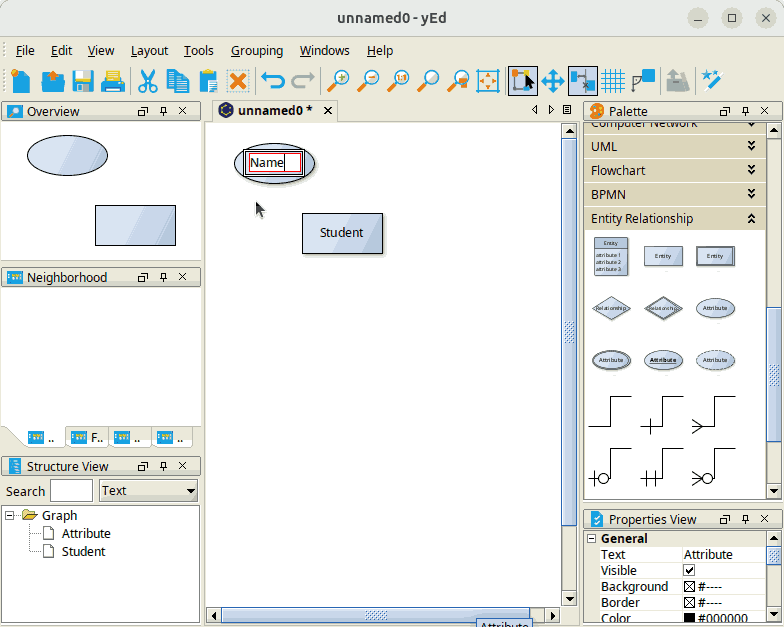
\includegraphics[width=0.48\linewidth]{\currentDir/yedErdEntitiesA09changeNameToName}}}%
%
\floatSep
%
\subfloat[][%
We changed the attribute name. %
Now we click on the connection symbol in the palette and drag it right onto the attribute.%
\label{fig:yedErdEntitiesA10changeNameChangedToNameSelectConnection}%
]{\tightbox{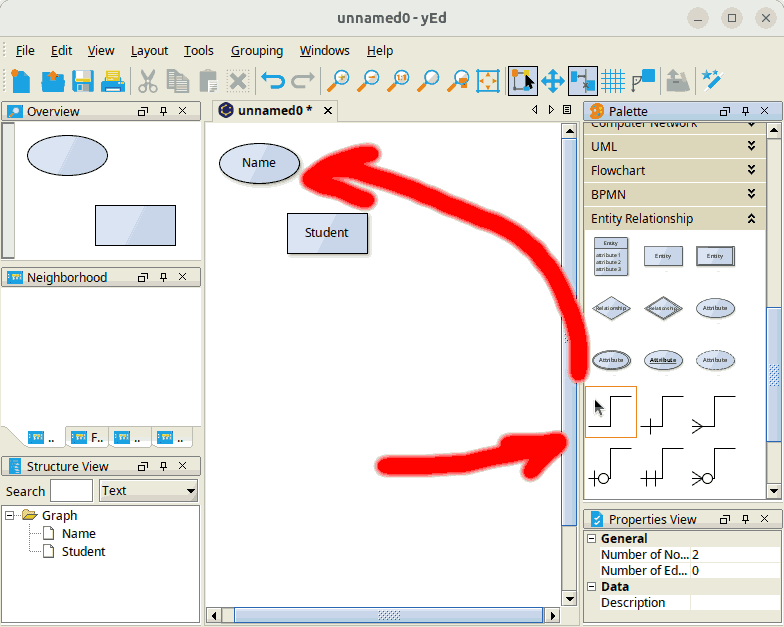
\includegraphics[width=0.48\linewidth]{\currentDir/yedErdEntitiesA10changeNameChangedToNameSelectConnection}}}%
%
\floatRowSep
%
\subfloat[][%
We drop the connection symbol onto the \emph{Name} attribute.%
\label{fig:yedErdEntitiesA11dragConnection}%
]{\tightbox{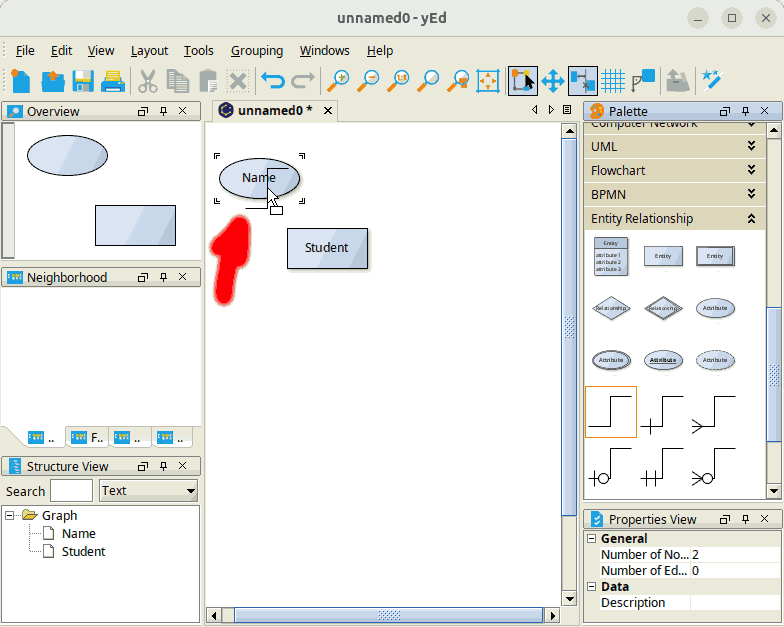
\includegraphics[width=0.48\linewidth]{\currentDir/yedErdEntitiesA11dragConnection}}}%
%
\floatSep
%
\subfloat[][%
We then click into the entity to connect the attribute \emph{Name} to the \emph{Student} entity.%
\label{fig:yedErdEntitiesA12connectToStudent}%
]{\tightbox{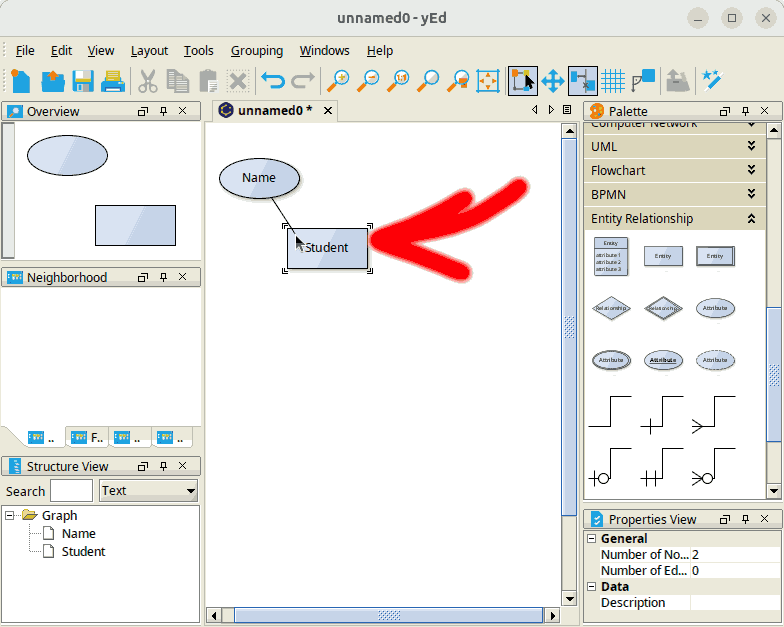
\includegraphics[width=0.48\linewidth]{\currentDir/yedErdEntitiesA12connectToStudent}}}%
%
\caption{Drawing an \pgls{ERD} for the \emph{Student} entity using \yEd~(Continued).}%
\label{fig:yedErdEntitiesA:B}%
\end{figure}%
%
\begin{figure}%
\ContinuedFloat%
\centering%
%
\subfloat[][%
The \emph{Name} attribute is now connected to the \emph{Student} entity.%
\label{fig:yedErdEntitiesA13connectedToStudent}%
]{\tightbox{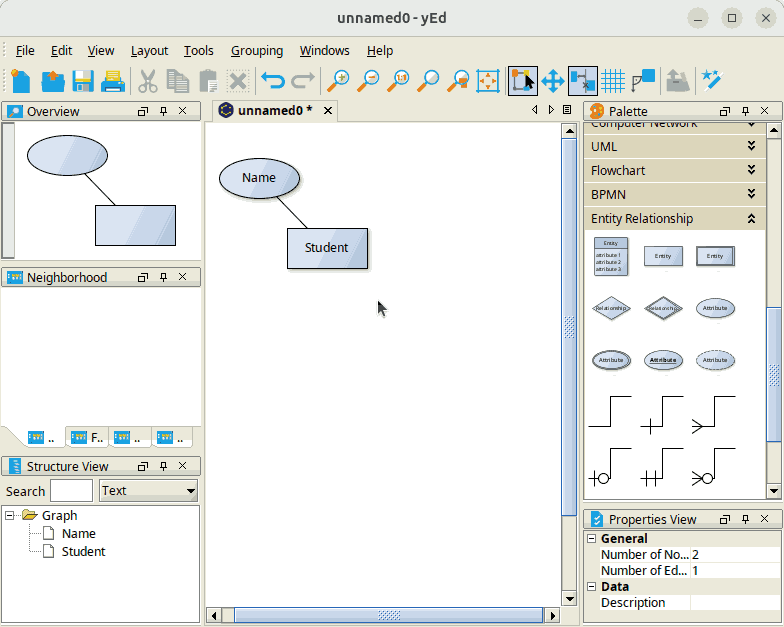
\includegraphics[width=0.48\linewidth]{\currentDir/yedErdEntitiesA13connectedToStudent}}}%
%
\floatSep%
%
\subfloat[][%
We add an attribute \emph{ID} in exactly the same way.%
\label{fig:yedErdEntitiesA14addedID}%
]{\tightbox{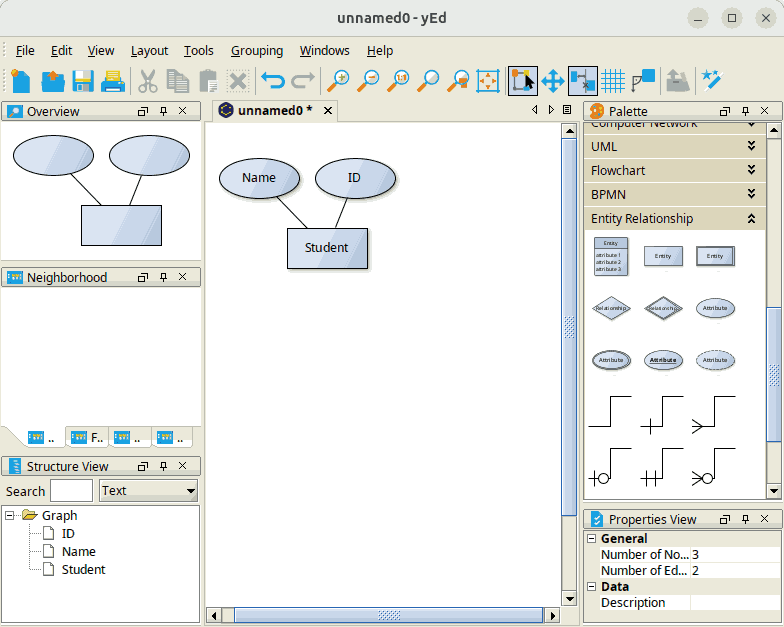
\includegraphics[width=0.48\linewidth]{\currentDir/yedErdEntitiesA14addedID}}}%
%
\floatRowSep
%
\subfloat[][%
We add several more attributes. %
Next, we click on the \menu{\underline{F}ile} menu.%
\label{fig:yedErdEntitiesA15addedAddrMobDoB}%
]{\tightbox{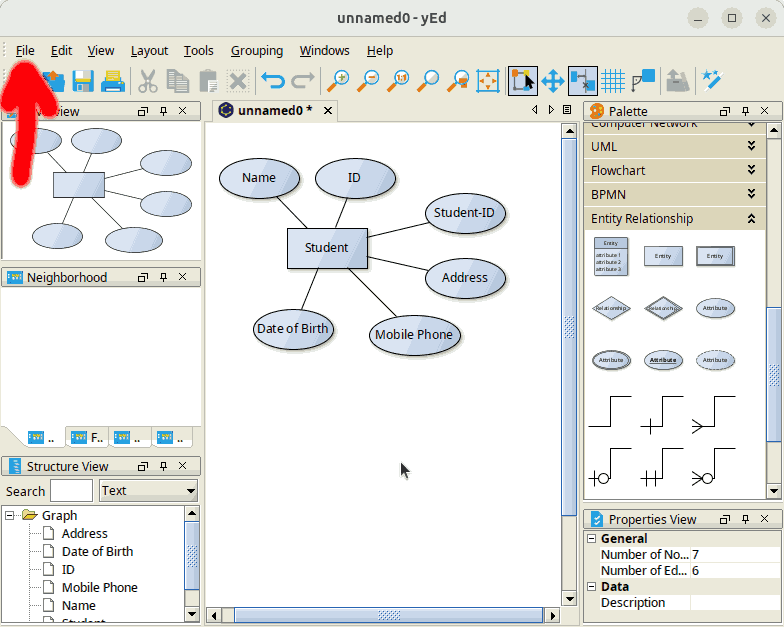
\includegraphics[width=0.48\linewidth]{\currentDir/yedErdEntitiesA15addedAddrMobDoB}}}%
%
\floatSep
%
\subfloat[][%
It is now time to save our document. %
We click on \menu{S\underline{a}ve As}.%
\label{fig:yedErdEntitiesA16saveAs}%
]{\tightbox{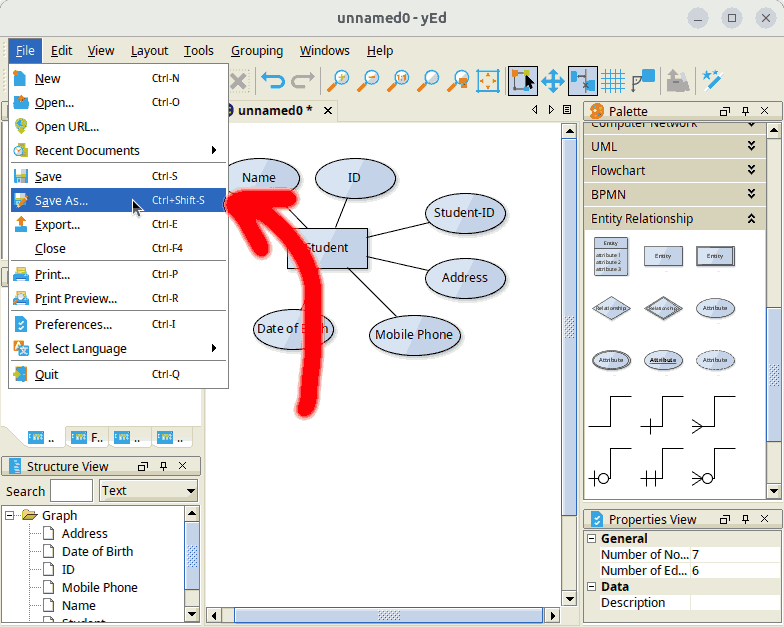
\includegraphics[width=0.48\linewidth]{\currentDir/yedErdEntitiesA16saveAs}}}%
%
\floatRowSep
%
\subfloat[][%
We save the diagram under the name \textil{erd_student_1} in the \textil{graphml} format by entering this name and clicking \menu{Save}.%
\label{fig:yedErdEntitiesA17saveAsErdStudent1}%
]{\tightbox{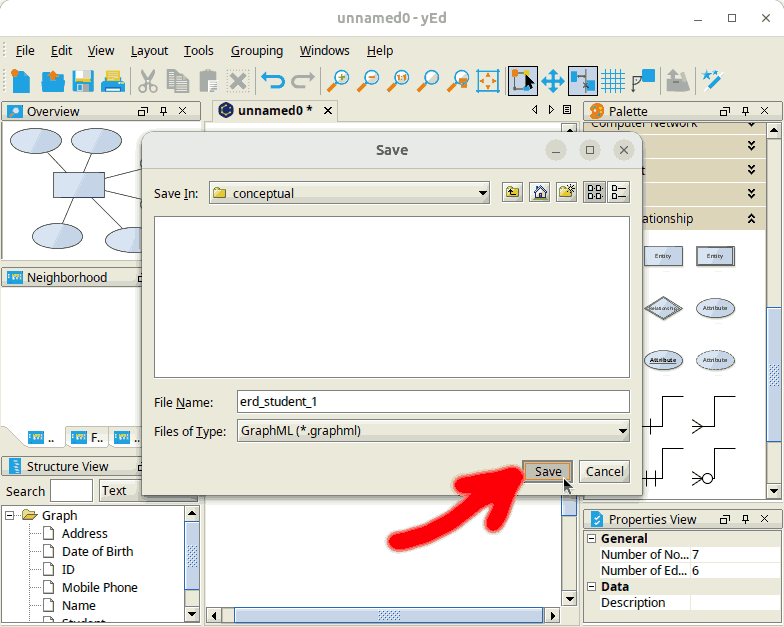
\includegraphics[width=0.48\linewidth]{\currentDir/yedErdEntitiesA17saveAsErdStudent1}}}%
%
\floatSep
%
\subfloat[][%
We can also store the diagram in a format that we can use in other documents. %
For this, we click on \menu{\underline{E}xport} in the \menu{\underline{F}ile} menu.%
\label{fig:yedErdEntitiesA18export}%
]{\tightbox{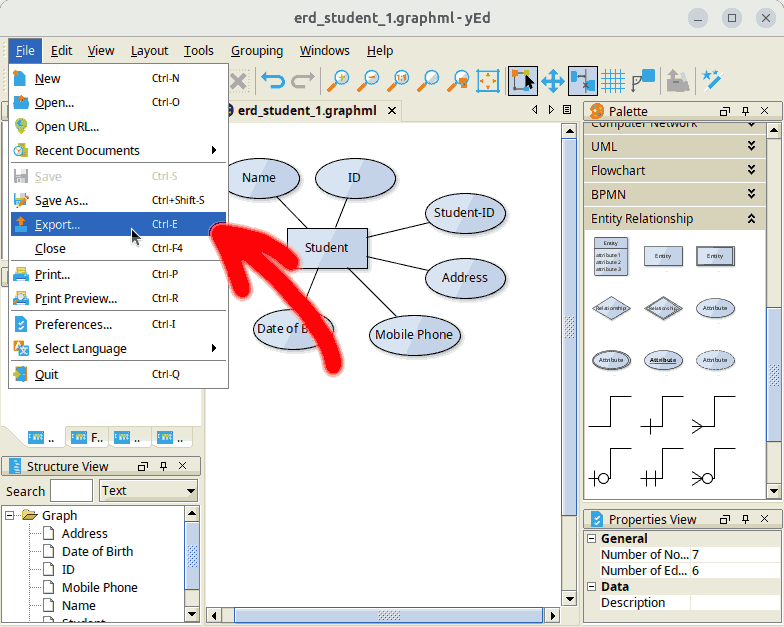
\includegraphics[width=0.48\linewidth]{\currentDir/yedErdEntitiesA18export}}}%
%
\caption{Drawing an \pgls{ERD} for the \emph{Student} entity using \yEd~(Continued).}%
\label{fig:yedErdEntitiesA:C}%
\end{figure}%
%
\begin{figure}%
\ContinuedFloat%
\centering%
%
\subfloat[][%
We choose to expert in the \pgls{SVG} format an click \menu{Save}.%
\label{fig:yedErdEntitiesA19exportToSvg}%
]{\tightbox{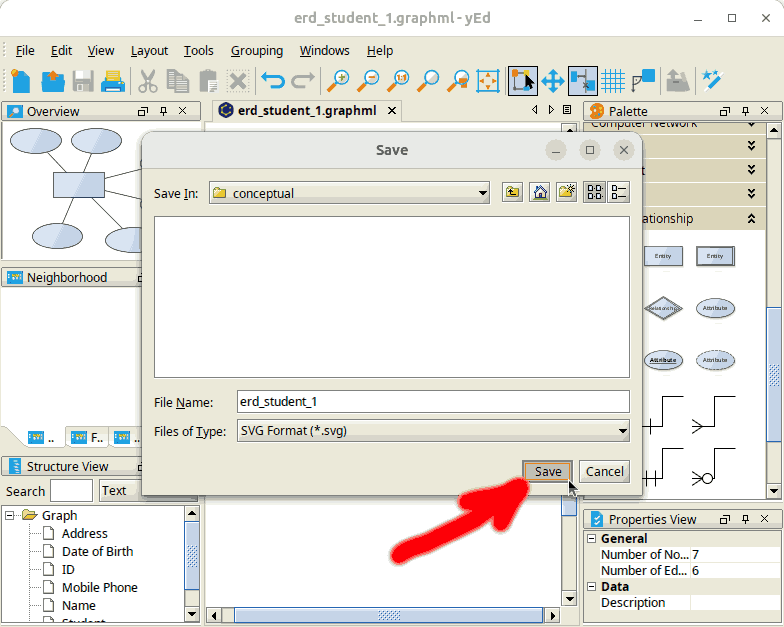
\includegraphics[width=0.48\linewidth]{\currentDir/yedErdEntitiesA19exportToSvg}}}%
%
\floatSep%
%
\subfloat[][%
We leave all settings as-is and click \menu{OK}.%
\label{fig:yedErdEntitiesA20exportToSvgDone}%
]{\tightbox{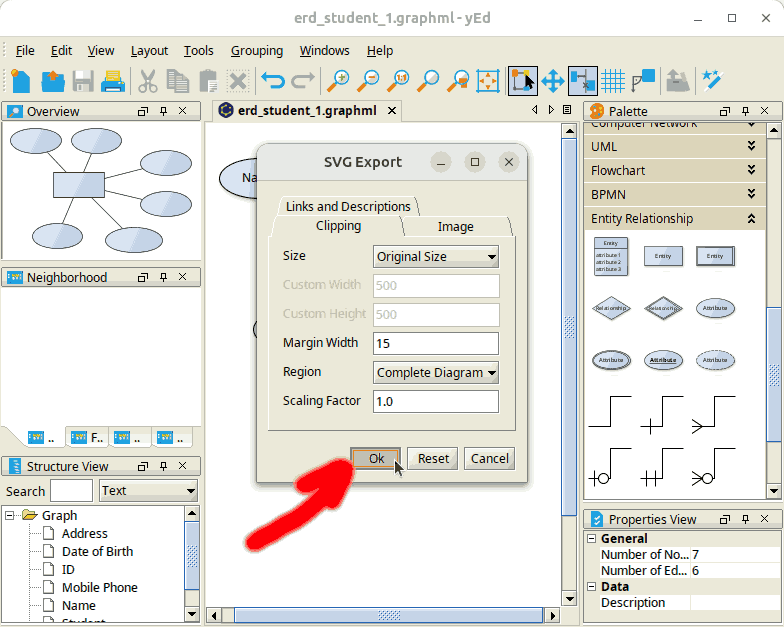
\includegraphics[width=0.48\linewidth]{\currentDir/yedErdEntitiesA20exportToSvgDone}}}%
%
\floatRowSep
%
\subfloat[][%
This produces this beautiful \pgls{ERD}.%
\label{fig:yedErdEntitiesA21erd}%
]{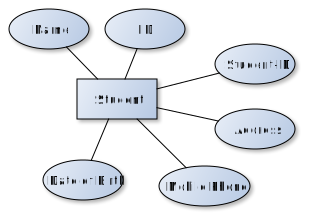
\includegraphics[width=0.6\linewidth]{\currentDir/yedErdEntitiesA21erd}}%
%
%
\caption{Drawing an \pgls{ERD} for the \emph{Student} entity using \yEd~(Continued).}%
\label{fig:yedErdEntitiesA:D}%
\end{figure}%
%

In the following sections, we will look at several different \pglspl{ERD}.
The goal of this course is to teach you \emph{actionable} knowledge.
So, while we will look at \pglspl{ERD}, we will also \emph{draw} them.
That, again, is fairly easy:
Once you understand the basic syntax, you can draw them with almost arbitrary drawing software.
Then again, this can also become tedious.
You could, for example, use the \softwareStyle{Draw} program which is part of \libreoffice, or a vector graphics program like \inkscape.
This would mean that you have to draw all the shapes of the diagrams independently, which would yield inconsistent designs and be generally tedious.
Then there are programs like \pgmodeler\ or \mysqlWorkbench\ which offer much better capabilities to draw \pglspl{ERD},
These tools, however, are bound to certain technologies, such as \postgresql\ and \mysql, respectively.
They would be useful for the development of logical models, but it feels awkward to apply them at a conceptual level, which should be technology agnostic.

After searching for a while, I have settled for \yEd~\cite{SG2015MDAWY,Y2011YGEM}.
\yEd\ is a free graph editor that offers a convenient ability to draw and layout \pglspl{ERD} while being entirely independent from any data model.
In \cref{sec:installingYed}, we provide instructions on how to obtain and install this program.
I will use it for all of the conceptual-level \pglspl{ERD} in the rest of the book.
As an example on how to use \yEd, we will give some instructions on how to draw the most simplest \pgls{ERD} with only a single entity inside in \cref{fig:yedErdEntitiesA:A}.
This program is rather easy to use, so after that example, we will assume that you can figure out how to draw more advanced \pglspl{ERD} on your own\dots
At least we do not just paint some \pglspl{ERD} and leave you entirely to your own devices when the time comes where you should draw some as well.

Before we really get into this, just a quick note:
In the context of \pglspl{ERD}, an \emph{entity type} are often called a \emph{entity}.
In other words, the meaning of the term \emph{entity} is shifted.
But let this not bother us too much.

The very first thing that we want to model is the entity (type) \emph{Student}.
From our requirements analysis, we know that students have names, they have an ID (issued by the government), they have a student ID (issued by our university), they have a mobile phone number, they have an address, and they have a date of birth.
So let us model this.

After installing \yEd\ as discussed in \cref{sec:installingYed}, we open it.
We scroll down the \menu{Palette} pane on the right-hand side until we find the \menu{Entity Relationship} tab.
We click on the tab and it opens in \cref{fig:yedErdEntitiesA01scrollToErd}, offering us all the symbols and connectors commonly used in \pglspl{ERD}.
Entity (types) in \pglspl{ERD} are represented by rectangles.
We can now click on the \menu{Entity} symbol and drag it into the empty document in \cref{fig:yedErdEntitiesA02entity}.
We dragged the entity symbol into the diagram document in \cref{fig:yedErdEntitiesA03dragEntity}.

Inside the rectangle, the name of the entity (type) is written.
Let's change it to \inQuotes{Student}.
We therefore double-click into the new entity symbol in order to edit its name in \cref{fig:yedErdEntitiesA04doubleClickName}.
The text inside is marked.
We change the entity name to \inQuotes{Student} and press \keys{\enter} in \cref{fig:yedErdEntitiesA05changeNameToStudent}.
The name has changed.

Let us now add the attributes of the \emph{Student} entity step by step.
Attributes are represented as oval bubbles in \pglspl{ERD} that are connected to their owning entities by straight lines.
We now click on the \menu{Attribute} symbol in the element palette in \cref{fig:yedErdEntitiesA06nameIsStudentSelectAttribute}.
We drag the attribute symbol into our document in \cref{fig:yedErdEntitiesA07dragAttribute}.

Of course, in \cref{fig:yedErdEntitiesA08doubleClickName}, we want to change its name as well.
So we double-click into it to change its name.
We want its name to be, well, \inQuotes{Name,} i.e., we want to create an attribute that represents the name of the student in \cref{fig:yedErdEntitiesA09changeNameToName}.
We successfully changed the attribute name in \cref{fig:yedErdEntitiesA10changeNameChangedToNameSelectConnection}.
The attribute, however, is still floating in the diagram all by itself.
Attributes belong to entities, so we need to attach it to the entity \emph{Student}.

We thus now we click on the connection symbol in the palette and drag it right onto the attribute.
We drop the connection symbol onto the \emph{Name} attribute in \cref{fig:yedErdEntitiesA11dragConnection}.
Our mouse cursor now marks the end of a connecting line and we can drag the connection to whatever object we want to.
We click into the entity rectangle to connect the attribute \emph{Name} to the \emph{Student} entity in \cref{fig:yedErdEntitiesA12connectToStudent}.
The \emph{Name} attribute is now connected to the \emph{Student} entity in \cref{fig:yedErdEntitiesA13connectedToStudent}.

We add an attribute \emph{ID} in exactly the same way in \cref{fig:yedErdEntitiesA14addedID}.
We then go on and add several more attributes, \emph{Student-ID}, \emph{Address}, \emph{Mobile Phone}, \emph{Date of Birth}, in \cref{fig:yedErdEntitiesA15addedAddrMobDoB}.
Notice that these are names that contain dashes and spaces, i.e., things that we would normally avoid when working with \sql.
But we are not working with \sql.
We are making a conceptual model.
We want this model to be easily readable and beautiful.
And it has to be.
Because we want to discuss it with our stakeholders.
So we do not need to heed to restrictions of a particular technology at this point in time.
Instead, we focus on readability.

Having finished drawing our very first \pgls{ERD}, it is time to save it.
Next, we click on the \menu{\underline{F}ile} menu.
We click on \menu{S\underline{a}ve As} in \cref{fig:yedErdEntitiesA16saveAs}.
We save the diagram under the name \textil{erd_student_1} in the \textil{graphml} format by entering this name and clicking \menu{Save} in \cref{fig:yedErdEntitiesA17saveAsErdStudent1}

We can open this file later in order to keep editing it.
However, we often want to also place the diagram into some document.
For this purpose, it makes sense to convert it to an image.
For this purpose, we click on \menu{\underline{E}xport} in the \menu{\underline{F}ile} menu in \cref{fig:yedErdEntitiesA18export}.
We choose to expert in the \glsreset{SVG}\pgls{SVG} format an click \menu{Save} in \cref{fig:yedErdEntitiesA19exportToSvg}.
In the dialog that pops up, we leave all settings as-is and click \menu{OK} in \cref{fig:yedErdEntitiesA20exportToSvgDone}.

This produces this beautiful \pgls{ERD} graphic shown in \cref{fig:yedErdEntitiesA21erd}.
Notice that we can also open the \pgls{SVG} graphic in other programs, such as \inkscape, to further edit and beautify it.
With this, we have completed our very first \pgls{ERD}.
(Although we did not yet really touch the \emph{Relationship} part symbolized by the \emph{R} in \pgls{ERD}.)

\usefulTool{yEd}{%
\yEd~\cite{SG2015MDAWY,Y2011YGEM} is a free graph editor that can be used to draw \pglspl{ERD}. %
It is useful for the conceptual modeling stage in \db\ design as discussed in \cref{sec:conceptualSchemaDesign}. %
Installation instructions are provided in \cref{sec:installingYed} and a small hands-on tutorial is given in \cref{sec:entitisAttrsErd}.%
}%
%
\FloatBarrier%
\endhsection%
%
